BPMax algorithm computes a four-dimensional sparse table $F(i_{1}, j_{1}, i_{2}, j_{2})$ shown in Figure~\ref{fig:bpmax_dependency}. The sparsity can be viewed as a triangle of triangular collections, where  $(i_{1}, j_{1})$-th triangle is denoted by $F(i_{1}, j_{1})$ and also called an inner triangle. The $(i_{2}, j_{2})$-th element of $F(i_{1}, j_{1})$ is denoted as  $F_{i_{1}, j_{1}, i_{2}, j_{2}}$.  
\begin{figure}[htbp]
\centerline{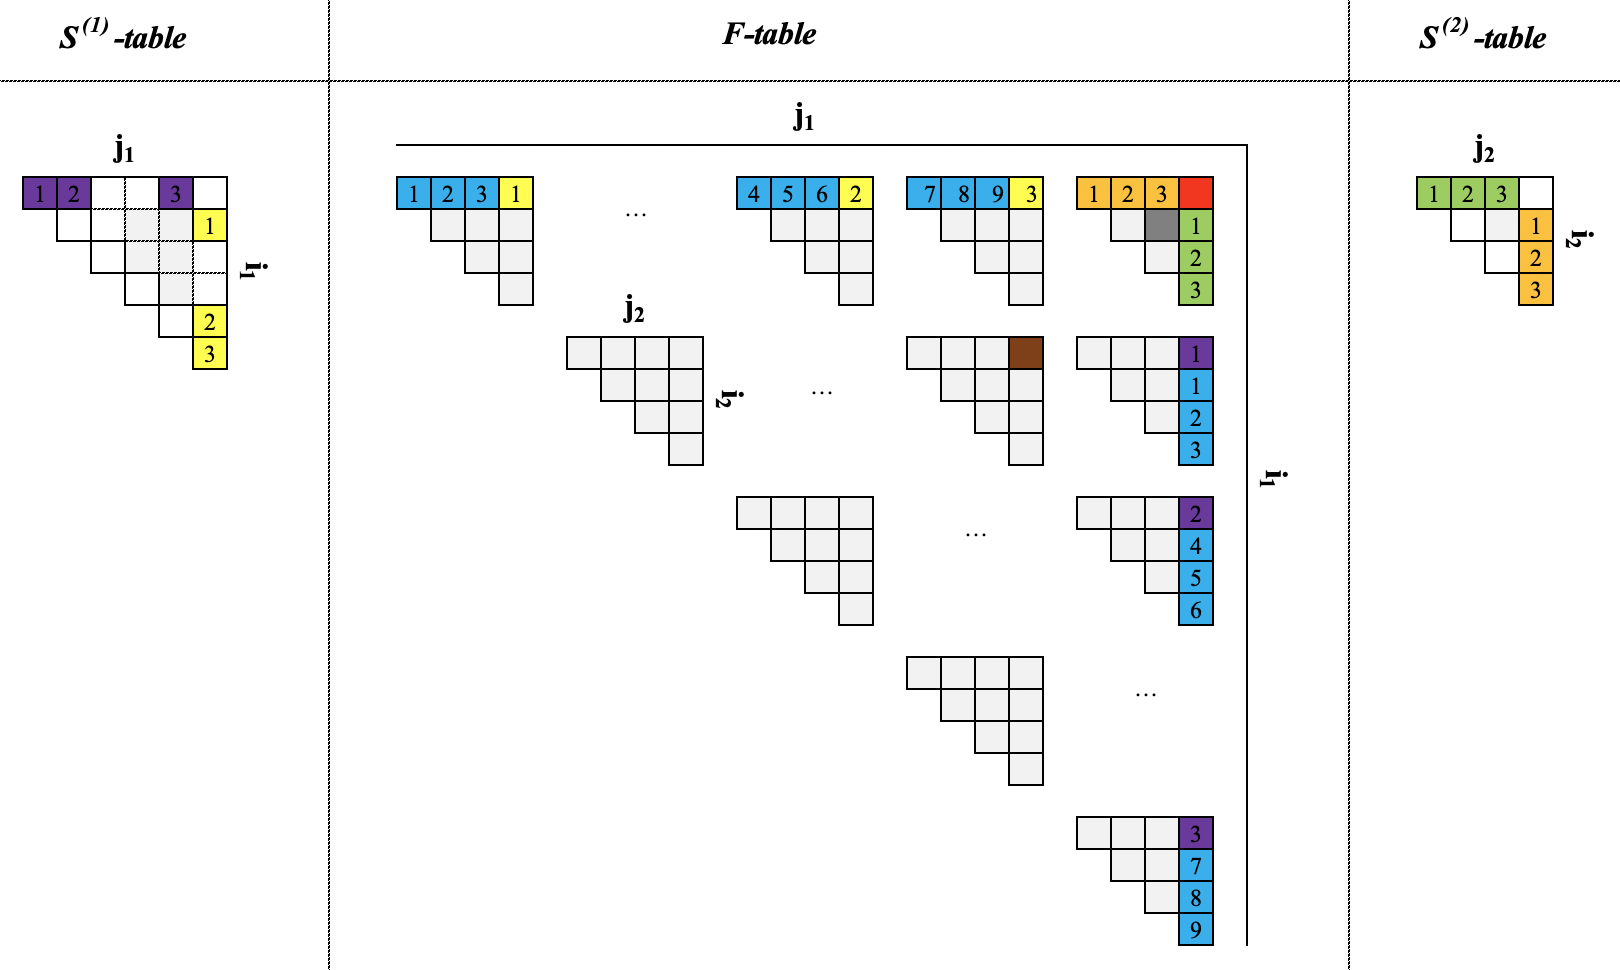
\includegraphics[scale=.30]{content/figures/bpm_dependency.png}}
\caption{BPMax dependency overview}
\label{fig:bpmax_dependency}
\end{figure}
Figure~\ref{fig:bpmax_dependency} shows the complete BPMax dependencies for an $F$-table element highlighted in red, which is dependent on all the blue, yellow, purple, orange, and green points of the $F$-table, $S^{(1)}$-table,  and $S^{(2)}$-table. Each color represents the computation of a particular reduction operation ($R^{0} - R^{4}$). %The blue, green, orange, purple, and yellow points contribute to the $R^{0}$, $R^{1}$, $R^{2}$, $R^{3}$, and $R^{4}$ respectively. 
All these reduction operations need to be completed to update the point highlighted in red. $R^{0}$ is the most compute-intensive ($\Theta({M^3N^3})$) reduction that uses the points outside the current triangle. E.g., to compute the $R^{0}$ for the red point,  the numbered blue points towards the left are added with the corresponding blue points towards the south, and then the max of all these values are computed. Now, $R^{3}$ and $R^{4}$ also use the elements from the external triangles as one of the operands and  $S^{(1)}$ as the other operand. E.g., the numbered yellow and purple points from the $F$-table are added with the corresponding yellow and purple points from the $S^{(1)}$-table, and then the max of yellow and purple results are computed to produce the $R^{3}$ and $R^{4}$, respectively. These two reductions have a complexity of $\Theta(M^3N^2)$. The remaining two reductions, $R^{1}$ and $R^{2}$, have a complexity of $\Theta(M^2N^3)$ and have intra-triangular dependencies. E.g., the numbered orange and green points from the $F$-table are added with the corresponding orange and green points from the $S^{(2)}$-table, and then the max of orange and green results are computed to produce the $R^{1}$ and $R^{2}$, respectively.



